% This is a modified version of Springer's LNCS template suitable for anonymized MICCAI 2025 main conference submissions. 
% Original file: samplepaper.tex, a sample chapter demonstrating the LLNCS macro package for Springer Computer Science proceedings; Version 2.21 of 2022/01/12

\documentclass[runningheads]{llncs}
%
\usepackage[T1]{fontenc}
% T1 fonts will be used to generate the final print and online PDFs,
% so please use T1 fonts in your manuscript whenever possible.
% Other font encodings may result in incorrect characters.
%
\usepackage{color}
\usepackage{graphicx,verbatim,multirow}
\usepackage[hidelinks]{hyperref}
\newcommand{\bluelink}[2]{\href{#1}{\textcolor{blue}{#2}}}
\usepackage{placeins}
% Used for displaying a sample figure. If possible, figure files should
% be included in EPS format.
%
% If you use the hyperref package, please uncomment the following two lines
% to display URLs in blue roman font according to Springer's eBook style:
%\usepackage{color}
%\renewcommand\UrlFont{\color{blue}\rmfamily}
%\urlstyle{rm}
%

\newcommand{\validationpanel}[2]{%
  \parbox[t]{\linewidth}{%
    \textbf{\large #1}\par\vspace{1.5mm}%
    \includegraphics[width=\linewidth]{#2}%
  }%
}

\begin{document}
%
\title{Local Validation and Workflow Integration of Pathology Foundation Models for Colorectal WSI Classification}
%\titlerunning{Abbreviated paper title}
% If the paper title is too long for the running head, you can set
% an abbreviated paper title here
%
\begin{comment}  %% Removed for anonymized MICCAI submission
\author{First Author\inst{1}\orcidID{0000-1111-2222-3333} \and
Second Author\inst{2,3}\orcidID{1111-2222-3333-4444} \and
Third Author\inst{3}\orcidID{2222--3333-4444-5555}}
%
\authorrunning{F. Author et al.}
% First names are abbreviated in the running head.
% If there are more than two authors, 'et al.' is used.
%
\institute{Princeton University, Princeton NJ 08544, USA \and
Springer Heidelberg, Tiergartenstr. 17, 69121 Heidelberg, Germany
\email{lncs@springer.com}\\
\url{http://www.springer.com/gp/computer-science/lncs} \and
ABC Institute, Rupert-Karls-University Heidelberg, Heidelberg, Germany\\
\email{\{abc,lncs\}@uni-heidelberg.de}}

\end{comment}

\author{Shahryar Noei\inst{1} \and
Marcia Raquel Pegoraro De Macedo\inst{1} \and
Margherita Zordan\inst{3} \and
Matteo Pozzi\inst{1} \and
Francesco Giuseppe Carbone\inst{3} \and
Flavio Ragni\inst{1} \and
Stefano Bovo\inst{1} \and
Gisella Sidoti\inst{3} \and
Mattia Barbareschi\inst{3} \and
Giuseppe Jurman\inst{1,2}}
\authorrunning{S. Noei et al.}
\institute{Fondazione Bruno Kessler, Data Science for Health, Trento, 38123, Italy
    \and
    Humanitas University, Department of Biomedical Sciences, Milan, 20072, Italy
    \and
    Unit of Surgical Pathology, Santa Chiara Hospital, Trento, 38122, Italy\\
    \email{snoei@fbk.eu}}  
\maketitle              % typeset the header of the contribution
%
\begin{abstract}
Clinical translation of computational pathology models requires both robust
validation across institutions and a defined strategy for integrating model
outputs into diagnostic workflows. We investigated this problem for
three-class colorectal whole-slide image classification into non-neoplastic tissue,
low-grade lesions, and high-grade lesions. Five pathology foundation models
were evaluated across 12 training and aggregation settings using public
development data and an independent local-hospital cohort. Representation
shift was measured repeatedly in the original foundation-model embeddings
and at successive attention-based multiple-instance learning layers. We then evaluated 
grade-based and confidence-based case allocation in a reader study with one expert and one novice 
pathologist with escalation when the novice diagnosis disagreed with the AI prediction. 
Foundation-model choice was the main determinant of local performance, whereas downstream setting variation
had a smaller effect. Run-level shift metrics were weak predictors of
performance loss, but foundation-model-level shift rankings corresponded to
sensitivity across downstream settings. In the reader study, AI alone
achieved an MCC of 0.834 and high-grade sensitivity of 81.1\%; the observed
human workflow after expert review of escalations achieved 0.808 and 71.6\%,
respectively. Confidence-based routing captured more AI errors than
grade-based routing (72.7\% versus 26.3\%), without increasing expert
workload, whereas displaying AI output did not improve pathologist
performance or alter escalation frequency. 

\keywords{Computational pathology \and Foundation models \and Domain shift
\and AI-assisted triage \and Clinical workflow integration}
% Authors must provide keywords and are not allowed to remove this Keyword section.

\end{abstract}
%
%
%
\section{Introduction}
Colorectal cancer is the third most frequently diagnosed cancer and the second leading cause
of cancer death worldwide \cite{bray2024global}. Most sporadic cases arise through adenomatous 
precursor lesions, for which histological grading, particularly the detection of high-grade dysplasia, 
informs surveillance and clinical management; high-grade dysplasia is associated with increased risk of subsequent 
advanced neoplasia \cite{toll2011highgrade}. 
As diagnostic volumes increase, cases are often first encountered by pathologists with 
variable experience, making efficient allocation to expert review clinically important. 
Triage systems could therefore support timely reporting while directing specialist attention
where it is most needed \cite{mayall2023triage}.

Computational pathology can support this by using weakly supervised learning to aggregate patch representations 
into slide-level predictions \cite{campanella2019clinical,lu2021dataefficient}. Pathology foundation models 
(FMs) provide general-purpose patch encoders with strong downstream performance across tasks \cite{campanella2025clinicalbenchmark,neidlinger2025benchmarking}. 

Despite these advances, local translation remains difficult. 
Models are often trained elsewhere and transferred to a target hospital, 
where differences in staining, processing, scanners, institutions, and patients can shift FM 
representations and reduce performance \cite{thiringer2026scanner,howard2021sitespecific}. 
Some studies have proposed compensating for domain shift through feature adaptation or alignment \cite{huang2025knowledge,liu2025hasd}, 
whereas others have investigated whether unlabeled feature-space distances can quantify shift and anticipate performance degradation \cite{poceviciute2023detecting}.
Finally, deployment requires not only robust model selection, but also a workflow strategy, 
such as routing cases by predicted risk or model uncertainty, with different implications for workload and safety \cite{geaney2023translation,vasey2022decide}.

In this study, we simulate the translation of a colorectal WSI classifier from public development data to 
a local hospital setting. We evaluate five pathology FMs across multiple downstream settings, 
measure both performance drop and representation shift from development to local cohorts, 
and test whether shift metrics explain performance loss or setting sensitivity. 
We then carry the selected model into a reader study comparing grade-based and 
confidence-based routing (Fig.~\ref{fig:study-overview}). 
Our results show that FM choice, more than downstream setting variation, drives local performance 
and stability; shift metrics are weak run-level predictors but informative at FM level; 
and confidence-based routing captures model errors better than grade-based routing.

Our main contributions are:
\begin{itemize}
    \item a systematic development-cohort and local-hospital evaluation of five pathology FMs
    across multiple training settings for three-class colorectal WSI
    classification;
    \item a repeated, layer-wise analysis of representation shift and its
    relationship with local-validation performance degradation and model stability;
    and
    \item a reader-study comparison of risk- and uncertainty-based case
    allocation in a human-supervised pathology workflow.
\end{itemize}

\begin{figure}[t]
\centering
\begin{minipage}[c]{0.55\textwidth}
\textbf{\large A}\par\vspace{1.5mm}
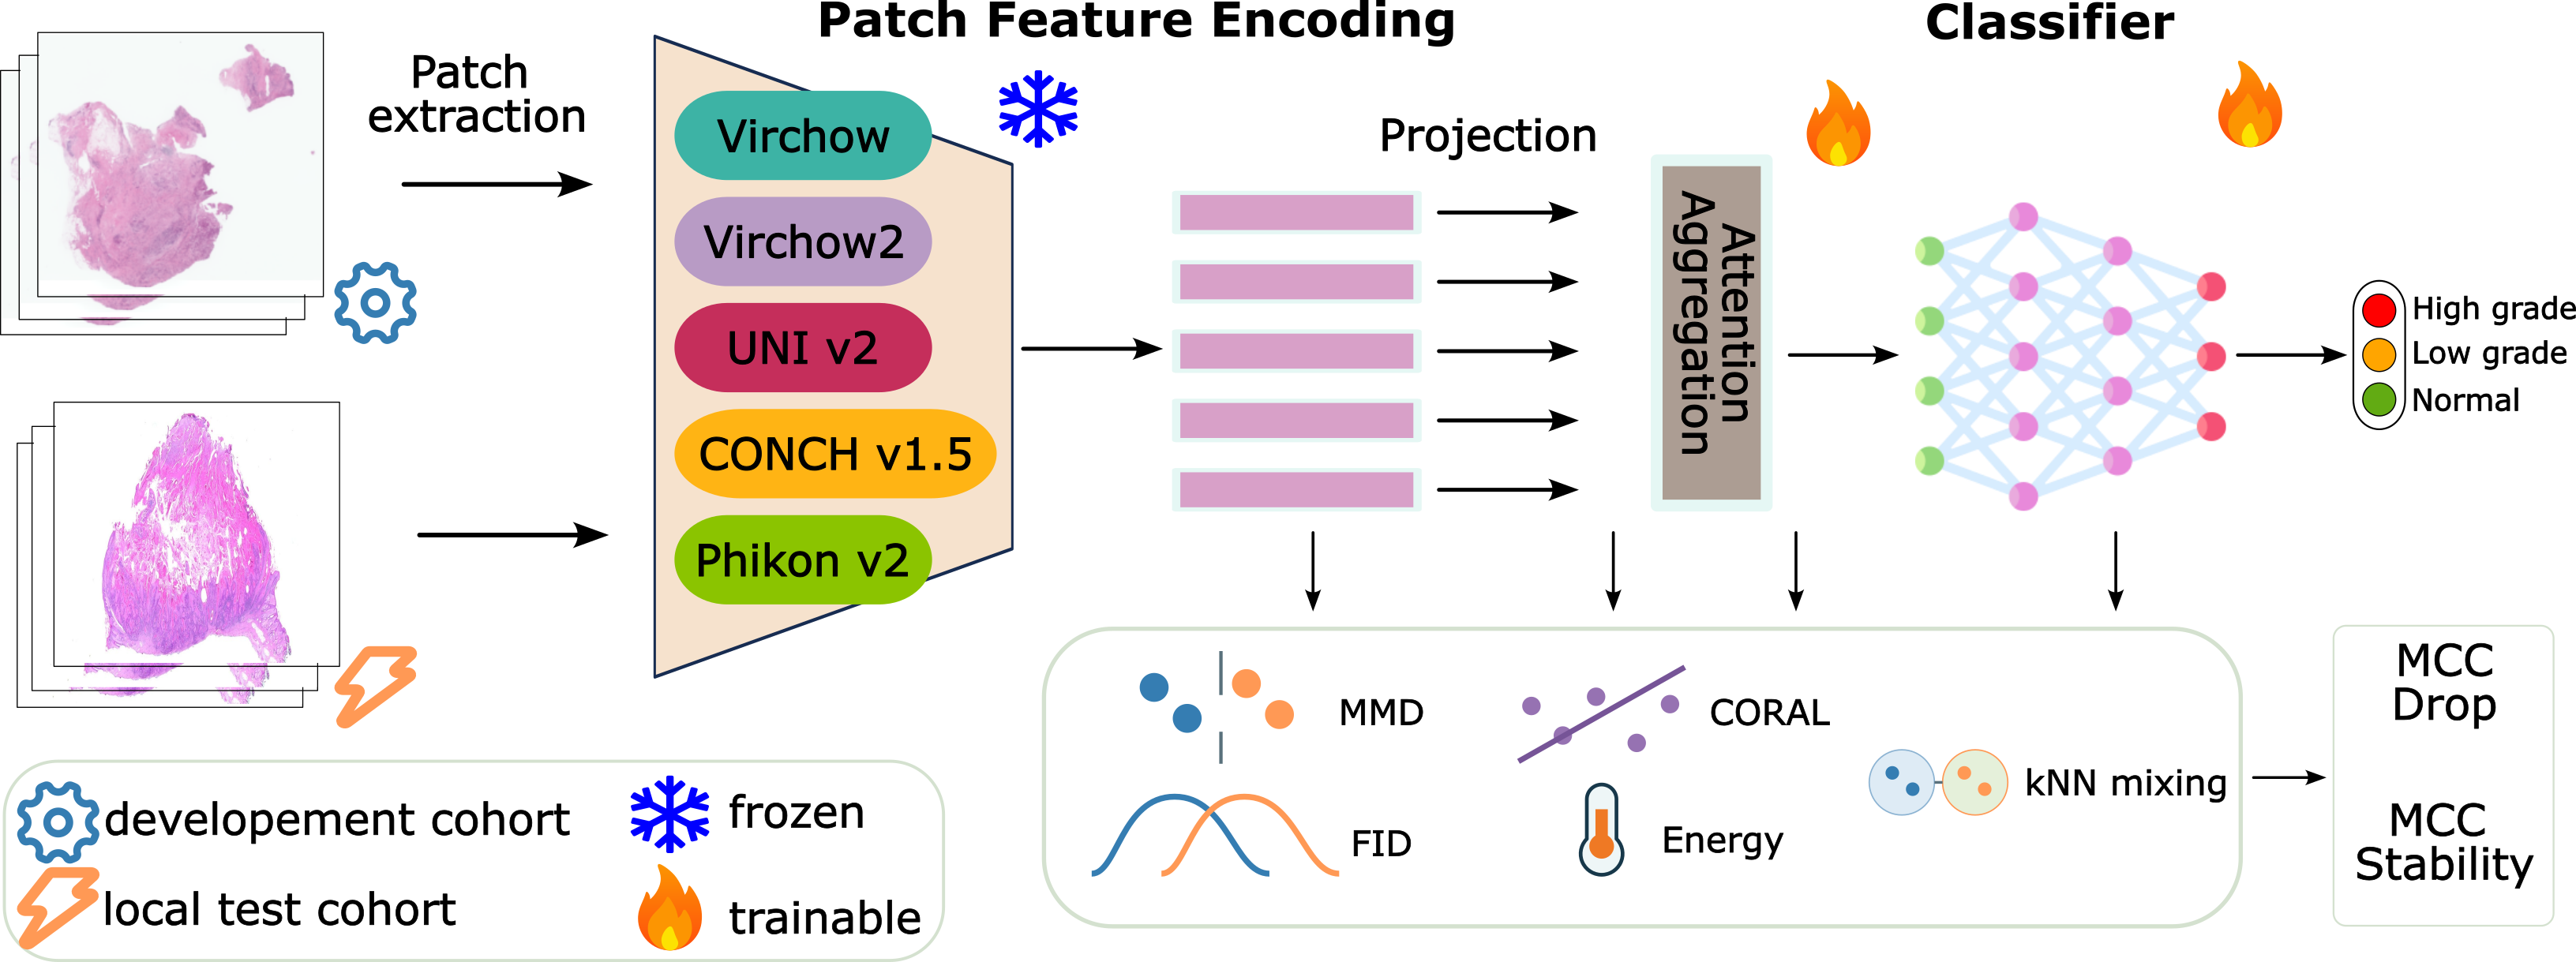
\includegraphics[width=\linewidth]{figures/panelA.png}
\end{minipage}\hfill
\begin{minipage}[c]{0.43\textwidth}
\textbf{\large B}\par\vspace{1.5mm}
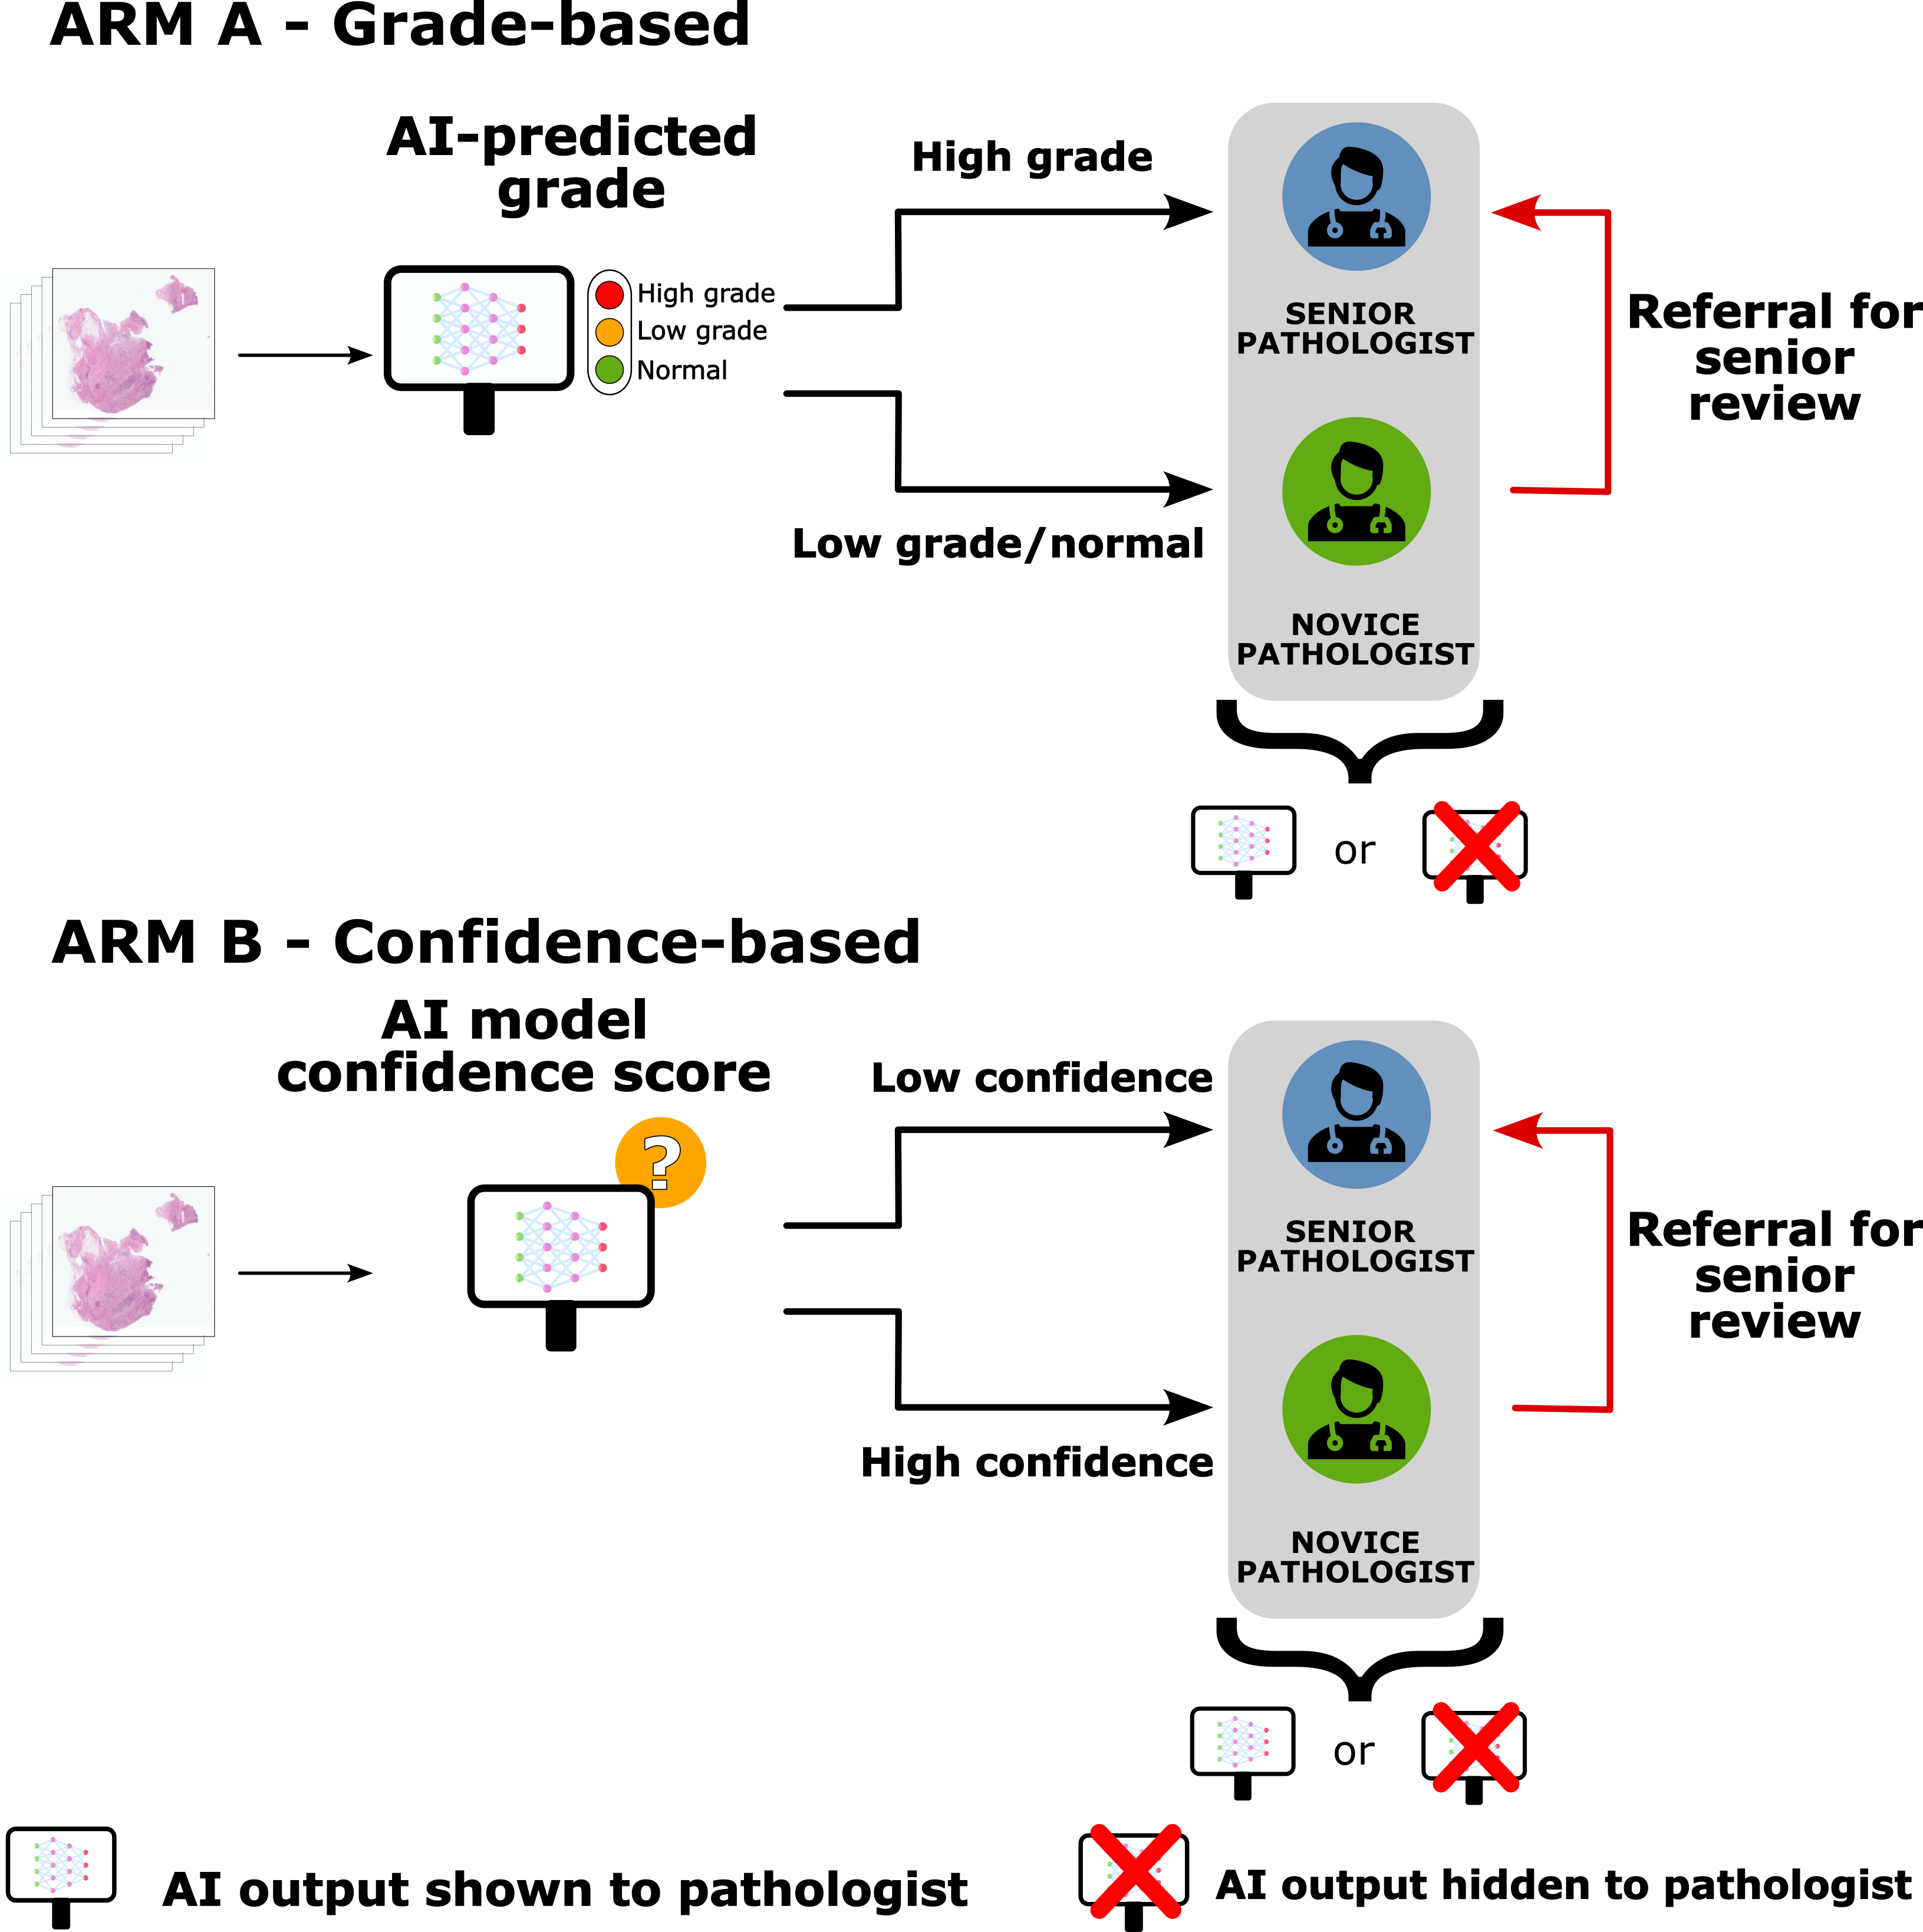
\includegraphics[width=\linewidth]{figures/triage_desgn.png}
\end{minipage}
\caption{Overview of the study.
\textbf{A}, Five pathology foundation models were evaluated using frozen
patch encoders and trainable ABMIL classifiers. Performance and
representation shift were assessed between the development and local
hospital cohorts using shift measures at different layers.
\textbf{B}, Reader-study design comparing grade-based and confidence-based
case allocation to senior and novice pathologists, with referral for senior
review upon disagreement with the AI prediction.}
\label{fig:study-overview}
\end{figure}

\section{Methods}
\subsection{Datasets}
We used the IMP Colorectal Sampling (IMP-CRS) dataset for model development, 
retaining its labels (847 non-neoplastic, 2,847 low-grade lesions, and 1,639 high-grade lesions) and original splits \cite{neto2024interpretable}. Local validation used 
152 colorectal WSIs from Santa Chiara Hospital, Trento: 43 non-neoplastic, 75 low-grade lesions, and 34 high-grade lesions. By IMP-CRS definitions, the high-grade class included high-grade dysplasia, intramucosal carcinoma, and invasive adenocarcinoma. 
The study was approved by the local ethical committee.

\subsection{Model Training}

Patch features were extracted with five pathology FMs: UNI v2 \cite{chen2024uni}, 
CONCH v1.5 \cite{lu2024conch}, Virchow \cite{vorontsov2024virchow}, Virchow2 \cite{zimmermann2024virchow2}, and Phikon v2 \cite{filiot2024phikon2}. 
Slide-level classification used ABMIL \cite{ilse2018attention}. 
We trained 60 models varying sampled patch count, attention architecture, hidden dimension, dropout, learning rate, and weight decay; for the full details refer to the \bluelink{https://github.com/Shahryar-Noei/colorectal-fm-local-validation}{project repository}. 
Models were trained with class-weighted cross-entropy, AdamW, and validation macro-F1 early stopping. WSI pre-processing, feature extraction, and ABMIL implementation used the Trident package \cite{zhang2025standardizing,vaidya2025molecular}.

\subsection{Performance and Representation-Shift Analysis}

Performance was measured by multiclass MCC, and performance drop was defined as 
$\mathrm{MCC}_{\mathrm{development}}-\mathrm{MCC}_{\mathrm{local}}$. 
Representation shift was quantified with MMD, Fr{\'e}chet distance, CORAL, energy distance, and $1-$k-nearest-neighbour domain mixing ($k=15$) 
after standardizing features with development-cohort statistics \cite{gretton2012kernel,heusel2017gans,sun2016deepcoral,szekely2013energy}. 
Shift was measured in the original FM mean-patch embedding and, for each ABMIL model, in mean pre-attention, 
attention-pooled, penultimate, and top-64 attention-weighted patch representations \cite{poceviciute2023detecting}. 
Repeat-specific MCC drops were computed on the same class-stratified samples of 80 development-test and 80 local-validation slides over 20 repetitions.

Associations with MCC drop were evaluated by Spearman correlation at run and FM levels. 
Setting sensitivity was defined as the standard deviation of MCC drop across training settings 
for each FM and repetition; grand-average FM-level analyses used one mean shift--sensitivity pair per 
FM with exact permutation testing. 
%Group comparisons used Mann--Whitney U or Kruskal--Wallis tests with Holm-corrected pairwise testing when appropriate; $p<0.05$ was considered significant.

\subsection{Reader Study}

The selected model was evaluated in a reader-study workflow simulation comparing two human--AI case-allocation 
strategies (Fig.~\ref{fig:study-overview}B). In Arm A, grade-based triage, cases with predicted high-grade probability higher than $0.20$ 
were assigned to the expert pathologist; all others went to the non-expert. In Arm B, confidence-based triage, 
uncertain cases were assigned to the expert, where uncertainty was defined as normalized predictive entropy at least $0.30$ or 
prediction margin was less than or equal to $0.20$. The routing thresholds were chosen as operational cutoffs to balance workload; 
sensitivity analyses showed that changes around these values did not substantially alter the main routing outcomes.
 Each assigned case was read once, with AI predictions shown for half of cases.

One gastrointestinal pathology expert and one pathology trainee participated. Novice cases were sent to expert review when the novice diagnosis 
disagreed with the AI prediction (escalation), and the expert diagnosis was considered final. The study included 300 cases: 
152 local-validation cases, 138 IMP-CRS development-test cases (added to increase sample size and balance the classes between the two arms). 
We also included 10 sessile serrated lesions (SSLs) from the local hospital, five in each arm, used as an out-of-distribution set (as the model has not seen this class). 
Readers also rated case difficulty on a scale of 1 to 5 (5 being the most difficult). 


\section{Results}
% Results will be inserted here.

\subsection{Model Validation Results}

Across the 60 ABMIL models, development-test MCC was consistently high, with FM
means ranging from 0.905 to 0.924 (Table~\ref{tab:validation}). Performance
decreased on the local validation cohort for every FM, where mean MCC ranged
from 0.724 to 0.762 and variability between runs increased. The distribution
of MCC drop remained primarily separated by FM rather than by the tested 
settings (Fig.~\ref{fig:validation-settings}A).
Univariable comparisons of training settings showed no consistent effect across the development and
local cohorts (Fig.~\ref{fig:validation-settings}B). Only learning rate showed one
nominal association with local-cohort MCC ($p=0.0373$), which was not mirrored in development performance.  
Notably, CONCH v1.5 had the lowest mean MCC on the development test
cohort, but achieved the highest mean MCC on the local validation cohort, the
smallest performance drop, and the lowest instability.

\begin{table}[!t]
\caption{Performance results for different foundation models.
Values are mean $\pm$ standard deviation across 12 settings per FM. Bold and
underlined values denote the best and second-best results, respectively.}
\label{tab:validation}
\centering
\small
\renewcommand{\arraystretch}{1.15}
\begin{tabular*}{\textwidth}{@{\extracolsep{\fill}}c|c|c|c@{}}
\noalign{\hrule height 1.0pt}
\textbf{\shortstack[c]{FM\\\strut}}
   & \textbf{\shortstack[c]{Development test\\cohort MCC}}
   & \textbf{\shortstack[c]{Local validation\\cohort MCC}}
   & \textbf{\shortstack[c]{MCC drop\\\strut}} \\
\noalign{\hrule height 0.5pt}
Virchow2   & $\mathbf{0.924\pm0.005}$ & $0.748\pm0.031$ & $0.176\pm0.031$ \\
Virchow    & $0.913\pm0.008$ & $0.748\pm0.035$ & $0.166\pm0.036$ \\
CONCH v1.5 & $0.905\pm0.007$ & $\mathbf{0.762\pm0.035}$ & $\mathbf{0.143\pm0.032}$ \\
UNI v2     & $\underline{0.920\pm0.011}$ & $0.724\pm0.065$ & $0.195\pm0.056$ \\
Phikon v2  & $0.913\pm0.006$ & $\underline{0.750\pm0.080}$ & $\underline{0.163\pm0.082}$ \\
\noalign{\hrule height 1.0pt}
\end{tabular*}
\end{table}

\begin{figure}[!h]
\centering
\begin{minipage}[t]{0.48\textwidth}
\validationpanel{A}{figures/figure1A_mcc_drop_portrait.pdf}
\end{minipage}\hfill
\begin{minipage}[t]{0.48\textwidth}
\validationpanel{B}{figures/figure1B_setting_effects_portrait.pdf}
\end{minipage}
\caption{Influence of FM choice and downstream training and aggregation
settings on validation performance. \textbf{A}, Development-to-local MCC drop
for all 60 trained models. Color denotes the FM; marker shape distinguishes the 12 downstream settings. 
\textbf{B}, Mean $\pm$ SEM MCC in the development test cohort (left)
and local validation cohort (right), stratified by individual settings.
Reported $p$ values are from two-sided Mann--Whitney U (MWU) or
Kruskal--Wallis (KW) tests, as appropriate.}
\label{fig:validation-settings}
\end{figure}

\begin{figure}[htb]
\centering
\begin{minipage}[t]{0.49\textwidth}
\textbf{\large A}\par\vspace{1.5mm}
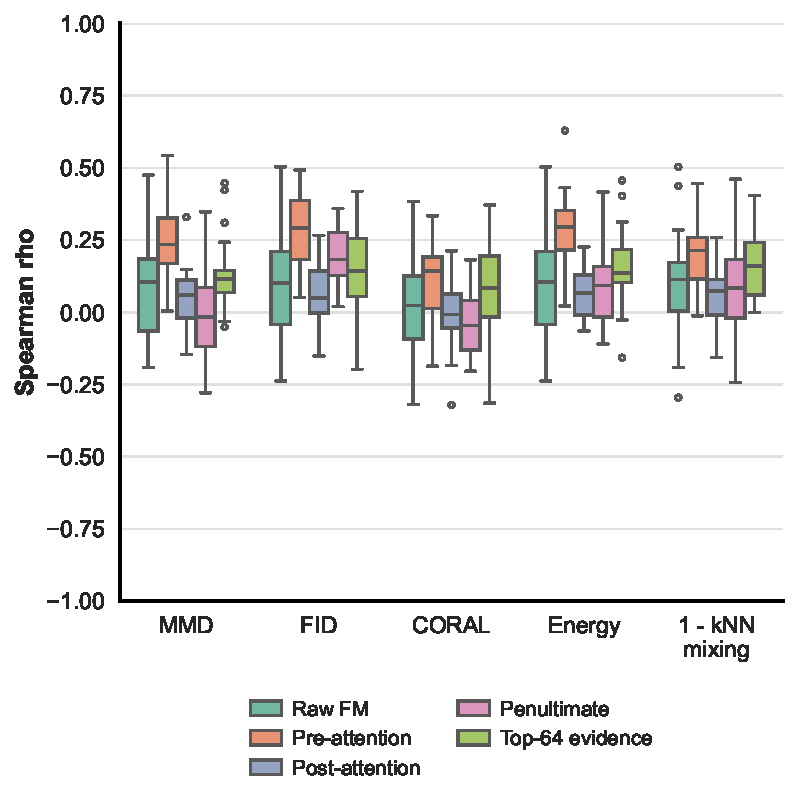
\includegraphics[width=\linewidth]{figures/panel2_shift_metric_repeat_correlation_boxplots_with_raw_fm.pdf}
\end{minipage}\hfill
\begin{minipage}[t]{0.49\textwidth}
\textbf{\large B}\par\vspace{1.5mm}
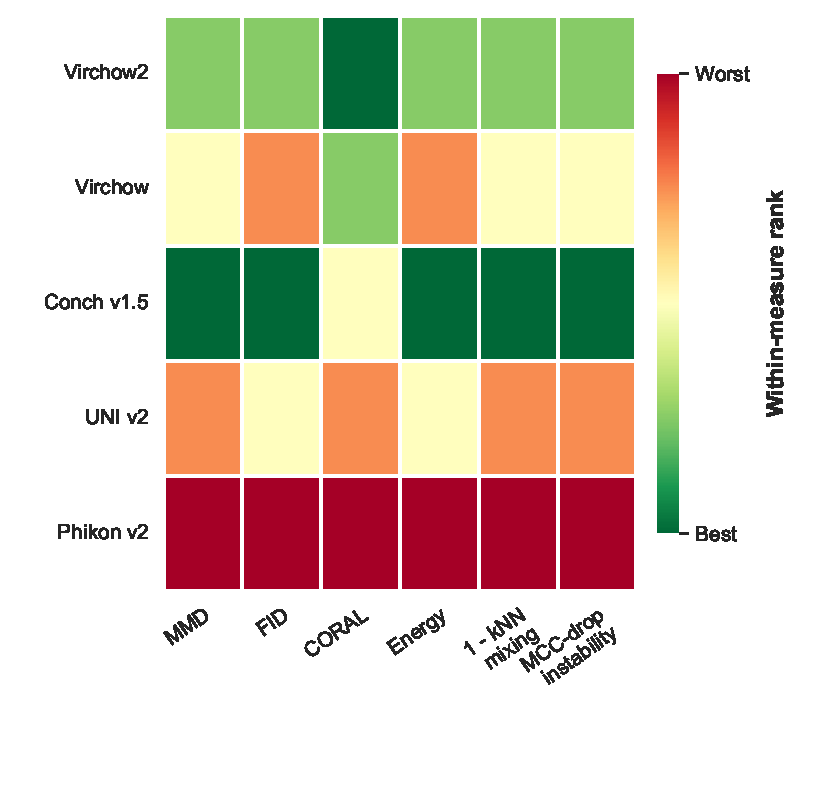
\includegraphics[width=\linewidth]{figures/fm_shift_and_instability_heatmap.pdf}
\end{minipage}
\caption{Representation shift and robustness. \textbf{A}, Run-level Spearman correlations between shift metrics 
and MCC drop across 20 matched repetitions. \textbf{B}, FM-level ranks of raw-feature shift and MCC-drop 
instability averaged across repetitions. Green indicates lower values and red higher values; 
instability is the standard deviation of MCC drop across the 12 settings within each FM.}
\label{fig:shift-analysis}
\end{figure}


For each repetition, each shift measurement was correlated with the
repetition-matched MCC drop across all 60 ABMIL runs.
Figure~\ref{fig:shift-analysis}A shows the resulting distribution of 20
Spearman correlations. Associations with MCC drop were generally weak.
The largest and most consistent correlations occurred in the mean
pre-attention representation: median $\rho$ was 0.24 for MMD, 0.29 for
Fr{\'e}chet distance, 0.14 for CORAL, 0.29 for energy distance, and 0.21 for
$1-$kNN mixing. Raw FM features had lower median correlations
($\rho=0.02$--0.11), while post-attention and penultimate representations
were not consistently more informative. Selecting the 64 patches with the
greatest positive attention evidence as proposed in \cite{poceviciute2023detecting} produced modest correlations, 
but did not outperform the pre-attention mean.


We next asked whether representation shift reflected \emph{FM-level robustness} rather than the MCC drop of 
individual runs. For each repetition and FM, we calculated setting sensitivity as the standard deviation of MCC 
drop across the 12 settings. We then averaged setting sensitivity and raw-feature shift metrics across the 20 repetitions 
to obtain one FM-level value for each measure (Fig.~\ref{fig:shift-analysis}B). 
CONCH showed the most favorable overall profile, with the lowest grand-average shift for 
 most metrics and the lowest setting sensitivity, whereas Phikon v2 showed the largest shift and greatest sensitivity. 
 Across FMs, larger raw-feature shifts generally aligned with greater setting sensitivity.



\subsection{Reader Study Results}
The highest performing CONCH model was carried forward to the reader study.
Across both arms, the AI alone achieved an MCC of 0.834 and high-grade (HG) sensitivity of
60/74 (81.1\%), compared with an MCC of 0.585 and HG sensitivity of
47/74 (63.5\%) for the initially assigned pathologists. Using the recorded
expert diagnosis for every escalated case increased workflow performance to
an MCC of 0.808 and HG sensitivity of 53/74 (71.6\%).

\begin{table}[!hbt]
\caption{Reader-study performance, AI visibility, and workload after
excluding SSL cases. HG values are sensitivity. ``Initial'' combines the
readers according to the initial allocation; ``final'' replaces escalated
novice diagnoses with the recorded expert diagnosis. Error capture is the
proportion of AI errors assigned directly to the expert.}
\label{tab:reader-arms}
\centering
\fontsize{8.6}{9.8}\selectfont
\renewcommand{\arraystretch}{1.08}
\setlength{\tabcolsep}{2.8pt}
\resizebox{\textwidth}{!}{%
\begin{tabular}{c|l|c|cc|cc|cc}
\noalign{\hrule height 1.0pt}
\textbf{Arm} & \textbf{Evaluation} & \textbf{$n$}
& \multicolumn{2}{c|}{\textbf{Overall}}
& \multicolumn{2}{c|}{\textbf{AI shown}}
& \multicolumn{2}{c}{\textbf{AI hidden}} \\
\cline{4-9}
& & & \textbf{MCC} & \textbf{HG}
& \textbf{MCC} & \textbf{HG}
& \textbf{MCC} & \textbf{HG} \\
\noalign{\hrule height 0.5pt}
\multirow{5}{*}{\textbf{A}}
& AI & 145 & 0.790 & 75.7\% & 0.827 & 80.0\% & 0.753 & 70.6\% \\
& Expert & 38 & 0.751 & 89.3\% & 0.839 & 93.8\% & 0.675 & 83.3\% \\
& Novice & 107 & 0.428 & 22.2\% & 0.374 & 0.0\% & 0.491 & 40.0\% \\
& Initial workflow & 145 & 0.572 & 73.0\% & 0.569 & 75.0\% & 0.581 & 70.6\% \\
& Final workflow & 145 & 0.781 & 67.6\% & 0.830 & 75.0\% & 0.730 & 58.8\% \\
\noalign{\hrule height 0.35pt}
\multirow{5}{*}{\textbf{B}}
& AI & 145 & 0.879 & 86.5\% & 0.897 & 94.7\% & 0.865 & 77.8\% \\
& Expert & 44 & 0.784 & 55.6\% & 0.797 & 80.0\% & 0.793 & 25.0\% \\
& Novice & 101 & 0.503 & 53.6\% & 0.477 & 42.9\% & 0.534 & 64.3\% \\
& Initial workflow & 145 & 0.604 & 54.1\% & 0.600 & 52.6\% & 0.610 & 55.6\% \\
& Final workflow & 145 & 0.835 & 75.7\% & 0.850 & 78.9\% & 0.820 & 72.2\% \\
\noalign{\hrule height 0.7pt}
\multicolumn{9}{c}{\textbf{Routing and expert workload}} \\
\noalign{\hrule height 0.35pt}
\textbf{Arm} & \textbf{Initial expert} & \textbf{Novice}
& \multicolumn{2}{c|}{\textbf{Escalations shown}}
& \multicolumn{2}{c|}{\textbf{Escalations hidden}}
& \textbf{Total expert load} & \textbf{Error capture} \\
\noalign{\hrule height 0.35pt}
A & 38 & 107 & \multicolumn{2}{c|}{14/54 (25.9\%)}
& \multicolumn{2}{c|}{18/53 (34.0\%)}
& 70/145 (48.3\%) & 5/19 (26.3\%) \\
B & 44 & 101 & \multicolumn{2}{c|}{17/51 (33.3\%)}
& \multicolumn{2}{c|}{13/50 (26.0\%)}
& 74/145 (51.0\%) & 8/11 (72.7\%) \\
\noalign{\hrule height 0.7pt}
\multicolumn{9}{c}{\textbf{OOD sessile serrated lesion recognition}} \\
\noalign{\hrule height 0.35pt}
\textbf{Arm} & \textbf{Assigned reader} & \textbf{OOD cases}
& \multicolumn{2}{c|}{\textbf{Initially recognized}}
& \multicolumn{2}{c|}{\textbf{Escalated}}
& \multicolumn{2}{c}{\textbf{Recognized after workflow}} \\
\noalign{\hrule height 0.35pt}
A & Novice & 5 & \multicolumn{2}{c|}{0/5 (0\%)}
& \multicolumn{2}{c|}{2/5 (40\%)}
& \multicolumn{2}{c}{0/5 (0\%)} \\
B & Expert & 5 & \multicolumn{2}{c|}{5/5 (100\%)}
& \multicolumn{2}{c|}{0/5 (0\%)}
& \multicolumn{2}{c}{5/5 (100\%)} \\
\noalign{\hrule height 1.0pt}
\end{tabular}
}
\end{table}

The two strategies produced nearly identical escalation rates
(Table~\ref{tab:reader-arms}) and similar total expert workloads:
70/145 cases (48.3\%) in Arm A and 74/145 (51.0\%) in Arm B. Their principal
difference was therefore the composition of the expert queue. Grade-based
routing sent 28/37 HG cases directly to the expert, compared with 9/37 under
confidence routing. Conversely, confidence routing captured a larger
proportion of AI errors in the initial expert queue (72.7\% versus 26.3\%;
Fisher exact $p=0.023$). Arm B had the higher final MCC, although the
bootstrap 95\% CI for the between-arm difference included zero
($\Delta=0.055$, 95\% CI $-0.061$ to 0.172). Final HG sensitivity also did
not differ significantly between arms ($p=0.607$).

Displaying the AI output did not improve initial pathologist MCC, HG
sensitivity, or escalation frequency (Table~\ref{tab:reader-arms}).
Overall escalation occurred in 29.5\% of shown and 30.1\% of hidden novice
cases ($p=1.00$), indicating that visibility did not suppress disagreement
or referral. Reader--AI agreement was also unchanged (74.8\% versus 74.5\%).
When the AI was wrong, readers recovered 5/13 shown and 6/17 hidden cases;
when it was correct, readers changed the prediction to an incorrect diagnosis
in 32/134 and 28/124 cases, respectively. Although final workflow MCC was numerically
higher for shown than hidden cases (0.839 versus 0.775), the bootstrap
confidence interval included no difference and the AI itself also performed
better on the shown subset.

Human and AI performance depended on when expert review occurred. Among the
82 cases assigned directly to the expert, expert MCC was 0.816
versus 0.755 for the AI: the expert corrected eight AI errors,
whereas the AI was correct in five cases missed by the expert. The AI
nevertheless had higher HG sensitivity (89.2\% versus 81.1\%). In contrast,
on the 62 escalated novice cases, the AI outperformed the expert adjudication
(MCC 0.808 versus 0.523; exact McNemar $p=0.021$) and had higher HG
sensitivity (75.0\% versus 50.0\%). Thus, escalation corrected many novice
errors, but expert review did not consistently improve upon the AI prediction
itself.

Perceived difficulty supported the confidence-routing rationale. Incorrect
diagnoses were rated more difficult than correct diagnoses overall
(median 3 [IQR 2--4] versus 2 [IQR 1--3], $p<10^{-7}$). Escalated cases were
also more difficult than non-escalated novice cases (median 3 versus 2,
$p=0.0025$). Finally, the SSLs were evaluated as a separate
out-of-distribution endpoint: all five assigned directly to the Arm B expert
were recognized as SSLs, whereas none of the five assigned initially to the
Arm A novice were recognized.

\section{Conclusion}
We evaluated the transfer and clinical integration of a colorectal WSI classifier
developed using an external public cohort and deployed on local hospital data.
Across 60 trained ABMIL models, FM selection had a greater influence on local
performance and robustness than variation in downstream training settings.
Unsupervised representation-shift measures did not reliably predict the
performance loss of an individual trained model; however, when aggregated by
FM, they identified broad differences in sensitivity to downstream settings.
Such measurements may therefore support FM-level robustness assessment.

The reader study further showed that implementation strategy was more
consequential than AI visibility alone. Grade-based routing prioritized HG cases,
whereas confidence-based routing captured substantially more AI errors with a
similar expert workload. Displaying the AI output did not improve MCC, HG
sensitivity, or escalation frequency. Expert adjudication corrected many novice
errors, but AI remained superior on the escalated case subset. Finally,
recognition of rare cases depended strongly on reader allocation. 
Because this pilot involved one expert and one novice pathologist, the findings
are preliminary and motivate larger multi-reader, multi-institution evaluations
of workflow-specific routing strategies. Overall,
safe clinical integration requires explicit local validation, routing aligned
with the clinical objective, and empirical evaluation of the entire human--AI
pathway, including the consequences of disagreement and escalation.

 %% removed for anonymized MICCAI submission.
    
    % The following acknowledgement and disclaimer sections can be removed for the double-blind review process.  If and when your paper is accepted, reinsert the acknowledgement and the disclaimer clause in your final camera-ready version.
    % IF you opted to include the acknowledgement and disclaimer sections, they will count towards the 8-page limit.

\begin{credits}
\subsubsection{\ackname} This study was funded by MUR under NRRP complementary investments, project D34H (PNC0000001), Spoke 2, CUP B53C22006170001.

\subsubsection{\discintname} The authors declare no competing interests.
\end{credits}

%
% ---- Bibliography ----
%
% BibTeX users should specify bibliography style 'splncs04'.
% References will then be sorted and formatted in the correct style.
%
\bibliographystyle{splncs04}
\bibliography{references}
\end{document}

